\documentclass[11pt]{article}

\usepackage{amsmath, amssymb}
\usepackage{graphicx}
\usepackage{geometry}
\usepackage{caption}
\usepackage{subcaption}

\geometry{margin=1in}

\title{A Finite-Difference Solver for the 2D Neutron Diffusion Equation}
\author{Your Name}
\date{\today}

\begin{document}

\maketitle

\section{Introduction}

Neutron diffusion models play a central role in reactor physics by approximating neutron transport in multiplying media. In this project, we develop a two-dimensional finite-difference solver for the steady-state neutron diffusion equation with spatially varying material properties. Both fixed-source and criticality formulations are considered, with numerical solutions obtained via sparse linear algebra methods.

\section{Governing Equations}

\subsection{Fixed-Source Diffusion}

The steady-state neutron diffusion equation in two dimensions is given by

\begin{equation}
- \nabla \cdot (D(x,y) \nabla \phi(x,y)) + \Sigma_a(x,y)\phi(x,y) = S(x,y),
\end{equation}

where:
\begin{itemize}
    \item $\phi(x,y)$ is the neutron flux,
    \item $D(x,y)$ is the diffusion coefficient,
    \item $\Sigma_a(x,y)$ is the absorption cross section,
    \item $S(x,y)$ is an external source.
\end{itemize}

Dirichlet boundary conditions $\phi = 0$ are imposed on the domain boundary.

\subsection{Criticality Eigenvalue Problem}

To model a multiplying system, we consider the one-group criticality equation:

\begin{equation}
- \nabla \cdot (D \nabla \phi) + \Sigma_a \phi = \frac{1}{k} \nu \Sigma_f \phi,
\end{equation}

where $\nu \Sigma_f$ represents neutron production via fission and $k$ is the effective multiplication factor.

This can be written as a generalized eigenvalue problem:

\begin{equation}
A \phi = \lambda F \phi, \quad \lambda = \frac{1}{k}.
\end{equation}

\section{Numerical Method}

The domain is discretized using a uniform Cartesian grid. A five-point finite-difference stencil is used to approximate the Laplacian:

\begin{equation}
\nabla^2 \phi \approx \frac{\phi_{i+1,j} - 2\phi_{i,j} + \phi_{i-1,j}}{h_x^2}
+ \frac{\phi_{i,j+1} - 2\phi_{i,j} + \phi_{i,j-1}}{h_y^2}.
\end{equation}

For spatially varying diffusion coefficients, harmonic averaging is used at cell interfaces to preserve flux continuity.

The discretization leads to a sparse linear system:

\begin{equation}
A \Phi = b,
\end{equation}

which is solved using SciPy's sparse direct solvers. The criticality problem is solved using a sparse generalized eigenvalue solver.

\section{Material Configurations}

Several heterogeneous configurations were considered:
\begin{itemize}
    \item Regions with varying diffusion coefficients to represent different materials,
    \item Localized high-absorption regions modeling control rods,
    \item Fissile regions with nonzero $\nu \Sigma_f$ for criticality analysis.
\end{itemize}

\section{Results}

\subsection{Fixed-Source Simulation}

Figure~\ref{fig:fixed} shows the neutron flux distribution for a heterogeneous medium with a localized source and absorber region.

\begin{figure}[h]
\centering
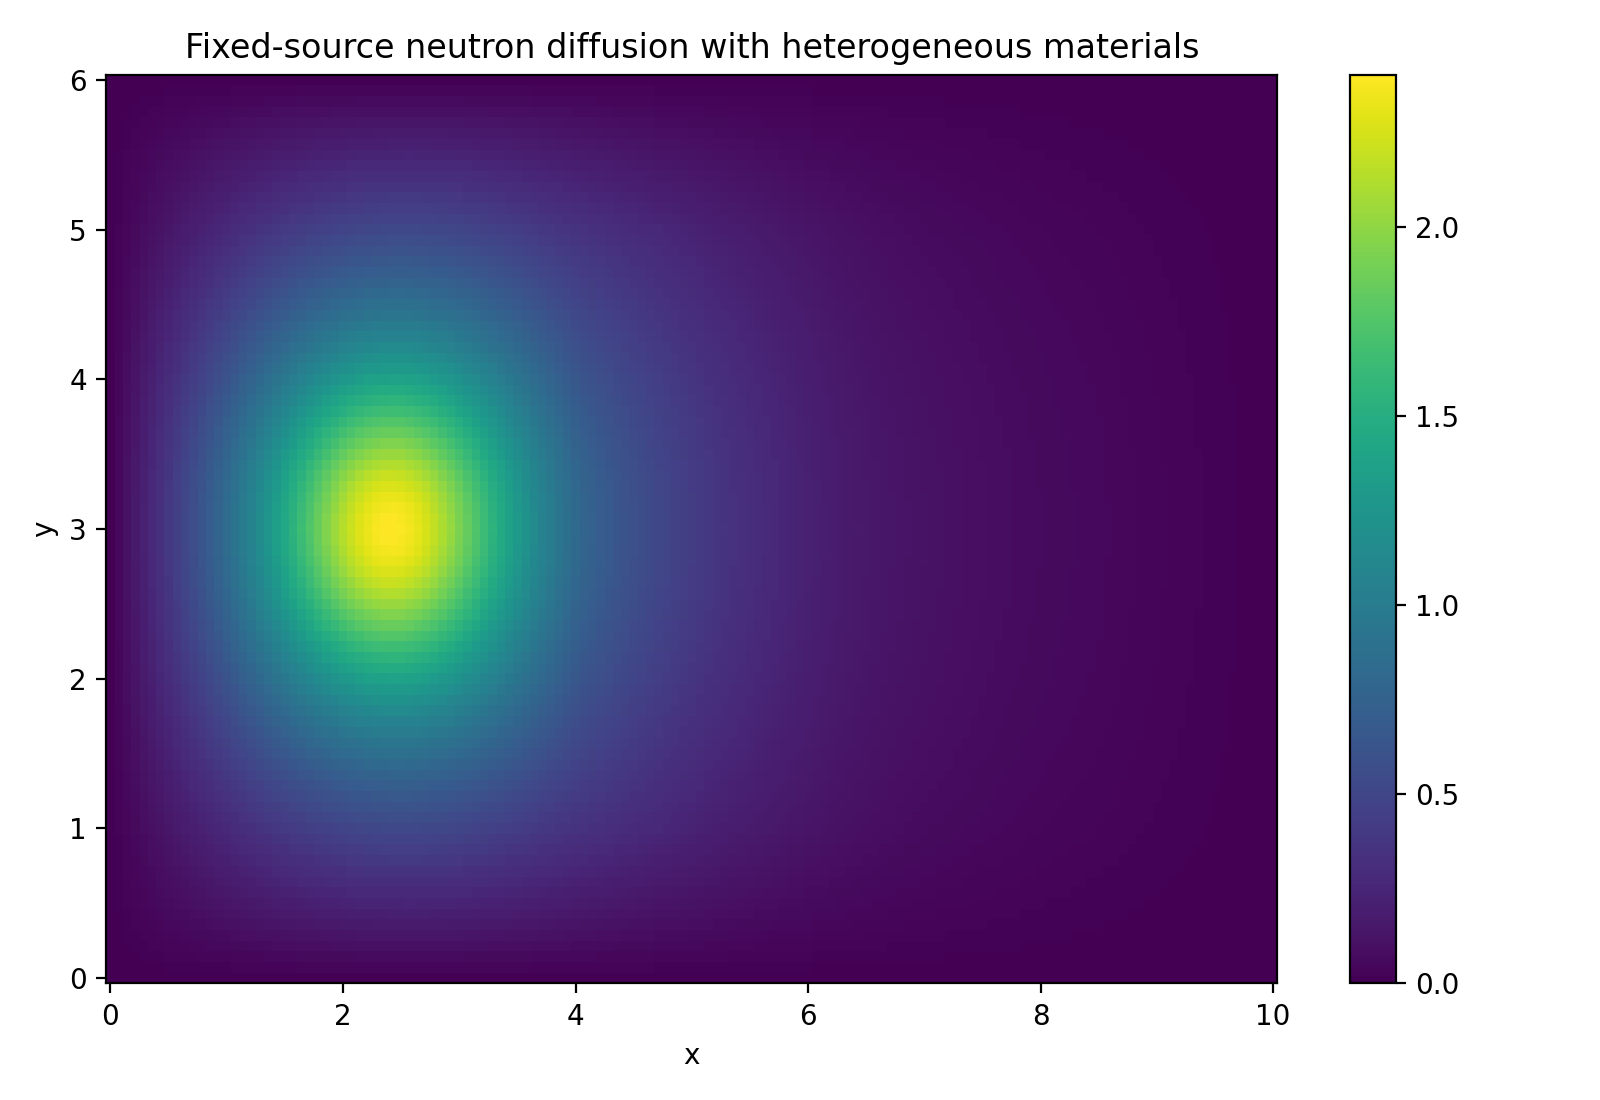
\includegraphics[width=0.8\textwidth]{figures/fixed_source_heterogeneous.png}
\caption{Neutron flux for a heterogeneous medium with source and absorber regions.}
\label{fig:fixed}
\end{figure}

The absorber region significantly reduces the local flux, while higher diffusion regions smooth the flux profile.

\subsection{Grid Refinement Study}

To assess numerical behavior, simulations were performed on increasingly refined grids.

\begin{figure}[h]
\centering
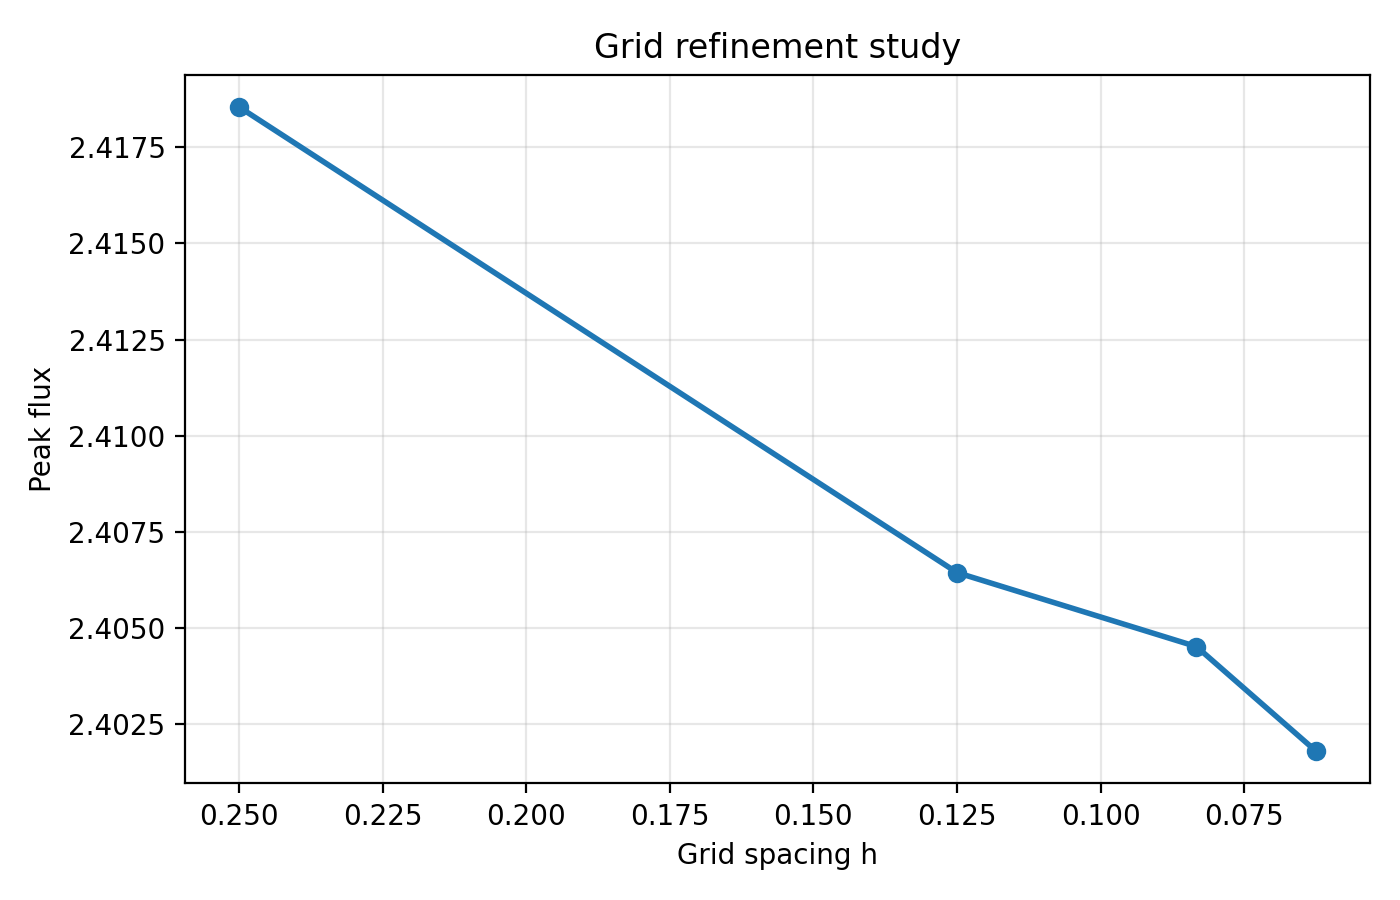
\includegraphics[width=0.7\textwidth]{figures/grid_refinement_peak_flux.png}
\caption{Peak flux versus grid spacing.}
\label{fig:refinement}
\end{figure}

As the grid is refined, the peak flux approaches a stable value, indicating convergence of the numerical solution.

\subsection{Criticality Analysis}

The dominant eigenmode and corresponding effective multiplication factor were computed.

\begin{figure}[h]
\centering
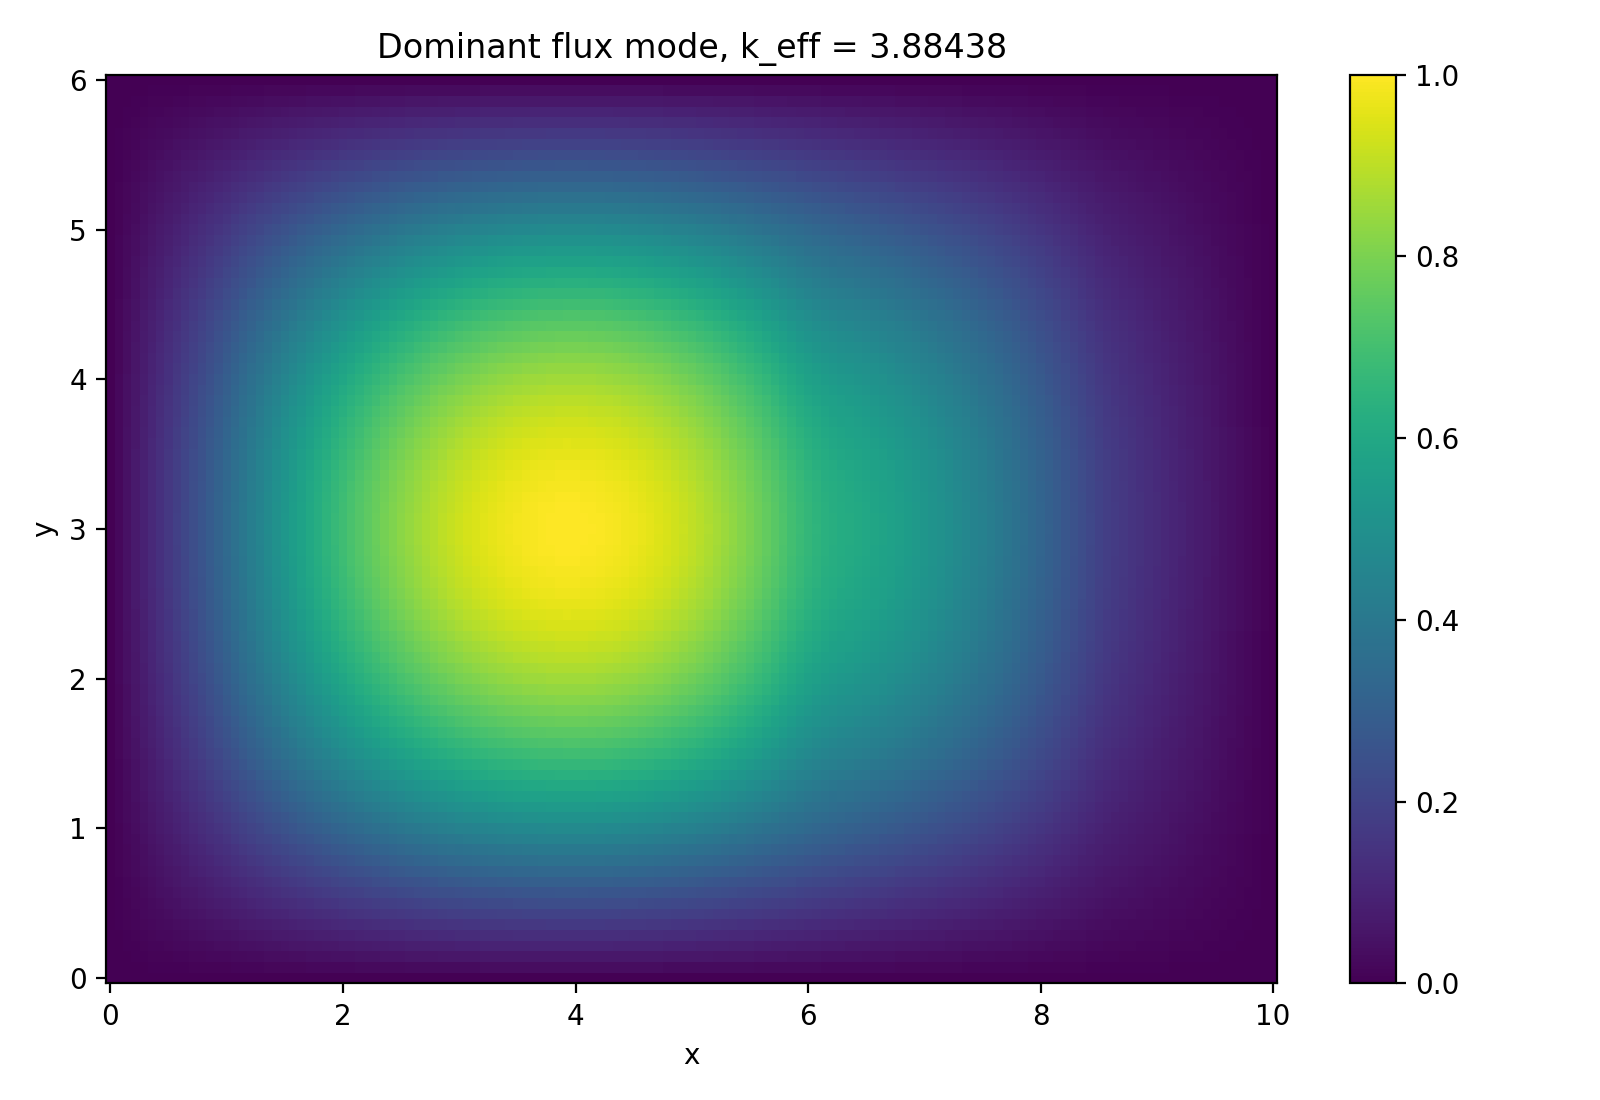
\includegraphics[width=0.8\textwidth]{figures/criticality_mode.png}
\caption{Dominant neutron flux mode for the criticality problem.}
\label{fig:criticality}
\end{figure}

The computed value of $k_{\mathrm{eff}}$ indicates whether the system is subcritical ($k<1$), critical ($k=1$), or supercritical ($k>1$). Spatial variations in absorption and fission properties strongly influence the flux shape.

\section{Discussion}

The results demonstrate the expected physical behavior:
\begin{itemize}
    \item Absorber regions suppress neutron flux locally.
    \item Higher diffusion coefficients lead to smoother spatial distributions.
    \item The eigenvalue solution reflects the balance between neutron production and loss.
\end{itemize}

The grid refinement study suggests that the finite-difference method provides consistent approximations as the mesh is refined.

\section{Conclusion}

A two-dimensional neutron diffusion solver was developed using finite-difference discretization and sparse linear algebra techniques. The implementation supports heterogeneous material properties and both fixed-source and eigenvalue formulations. The results align with expected physical behavior and demonstrate the capability of the model to capture key aspects of neutron transport.

\section{Future Work}

Potential extensions include:
\begin{itemize}
    \item Implementation of vacuum or Robin boundary conditions,
    \item Multigroup diffusion models,
    \item Time-dependent neutron diffusion,
    \item Comparison with finite-element methods.
\end{itemize}

\end{document}